%\documentclass[aip, jcp, preprint]
\documentclass{article}[12pt]
\usepackage{graphicx}
\usepackage{amsmath}
\usepackage[margin=1in]{geometry}

\title{23andMe Product Sales Analysis}
\author{Ryan Applegate}
\begin{document}
\maketitle

\section{Data Background and Visualization}

Time stamped sales data by gender is studied with some minimal python scripts. 
Processing the data involved combining 50 .csv files into arrays for the
 following items: dates, male customers sales, female customer sales, and
sales by time of day. Questions
 regarding total sales can be addressed by combining the
male and female lists. A visual for all sales is shown in the plot below.

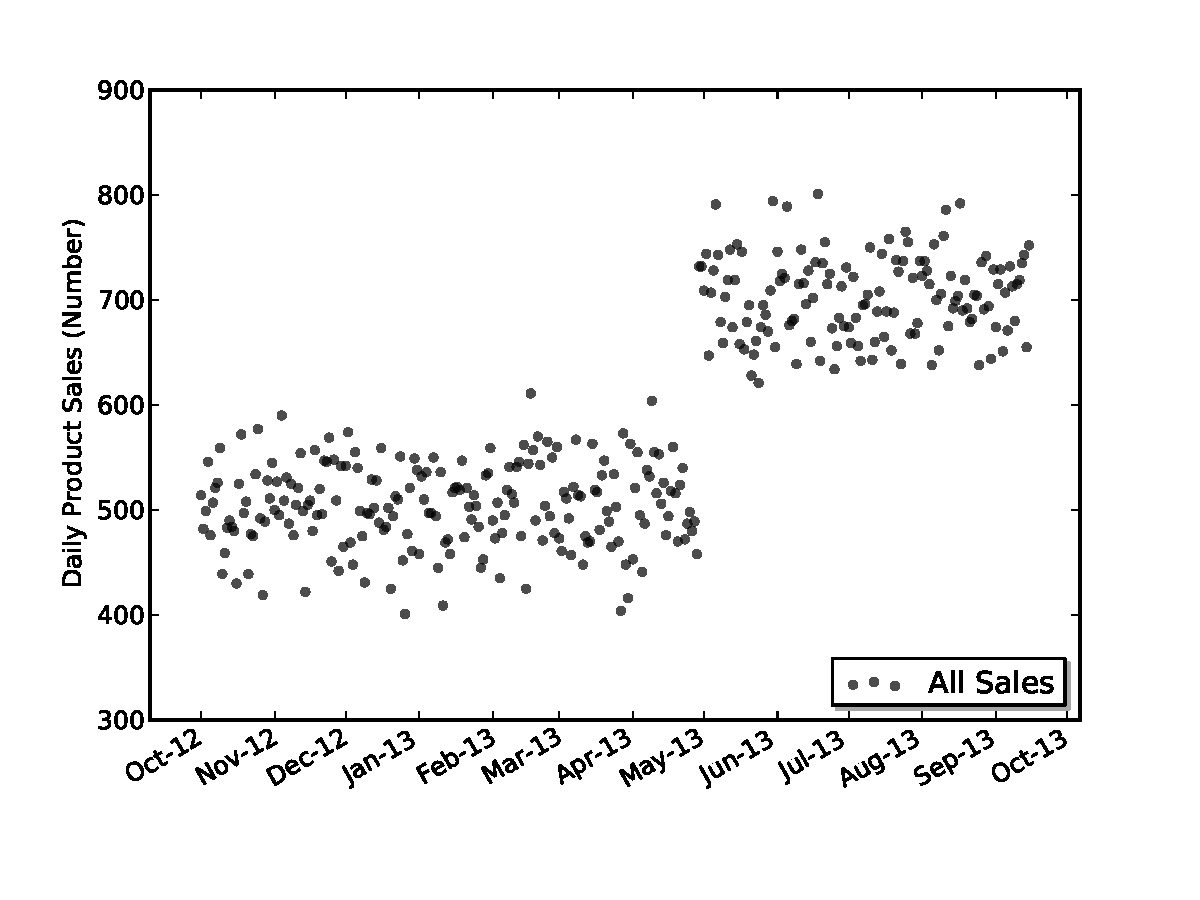
\includegraphics[scale=0.7]{../DailySalesNumbersFINAL.pdf}

\section{Jump in Sales and p-value}
The evidence from the Daily Product Sales graph shows a distinct jump some time
between Apr-13 and Jun-13. I hypothesized the data are well modeled by
two flat lines, each with their
own mean $\mu_1,\mu_2$ (this is the y-intercept of the line) and their own variance $\sigma^2_1, \sigma^2_2$. To locate
the jump, I iterated through the possible date splits, recalculating statistics
 at each possibile
split date. Given the statistics for all possible splits, I picked the one that
minimized the sum of the two distribution variances:

\begin{equation}
\sigma_{joint}^2 = \sigma_1^2 + \sigma_2^2.
\end{equation}

\noindent
{\bf The minimum of this function gives a date of April 29, 2013 for the sudden change in
daily sales.}

Calling the date for which the jump occurs N, one calculates p-values as new
 sales data arrive using a single normal distribution with
 $\mu=504.4,\sigma=39.9$. Concretely, the test hypothesis supposes there are 
two flat lines (with normal variation) to which sales belong, one before the jump and one after.
 The null hypothesis supposes all sales can be modeled by a single distribution
based on past data up to the current day. On the $N-1$ day, the daily sales is $489$ with a p-value of $0.70$. Given the null hypothesis, there is a $70\%$ chance
 of observing a fluctuation in sales at least as large as on the $N-1$ day.
 {\bf On day $N$ the daily sales is $732$ and the p-value is $1.2\times10^{-8}$, significant enough to reject the null hypothesis of a single normal distrubtion, and 
accept the test hypothesis that there are two distinct distributions.}

The choice of the normal distribution is conservative and warrants some discussion.
To select a distribution, I generated random samples
using normal, uniform, and Poisson distributions constructed directly from the measured data mean and variation. A uniform distribution gives
 a $N^{th}$ day p-value of exactly zero which seems overly strong for a sales distribution. Working against a uniform distribution still, the data are centered more strongly around the mean than uniformly between the minimum and maximum from the data.

 The Poisson distribution seems a natural choice because the sale of a product is
bounded from below (can't have a  negative sale in this model) but the Poisson distribution constructed from the measured mean and variance is a poor visual fit.
Additionally, the standard deviation of the data before and after the jump are nearly
equal. The variance in the Poisson distribution would have to grow with the mean of the data. The normal distribution is less than ideal visually yielding more spread than are present in the data. However, the normal model does capture the obvious visual jump and the fact that the values vary signficantly from the pre-jump mean.

\section{Male/Female Sales Impact on the Jump}

One may expect that gender plays a role in sales. To get an idea of this effect,
I plot the components of total sales, namely the male and female sales alongside
the total sales.


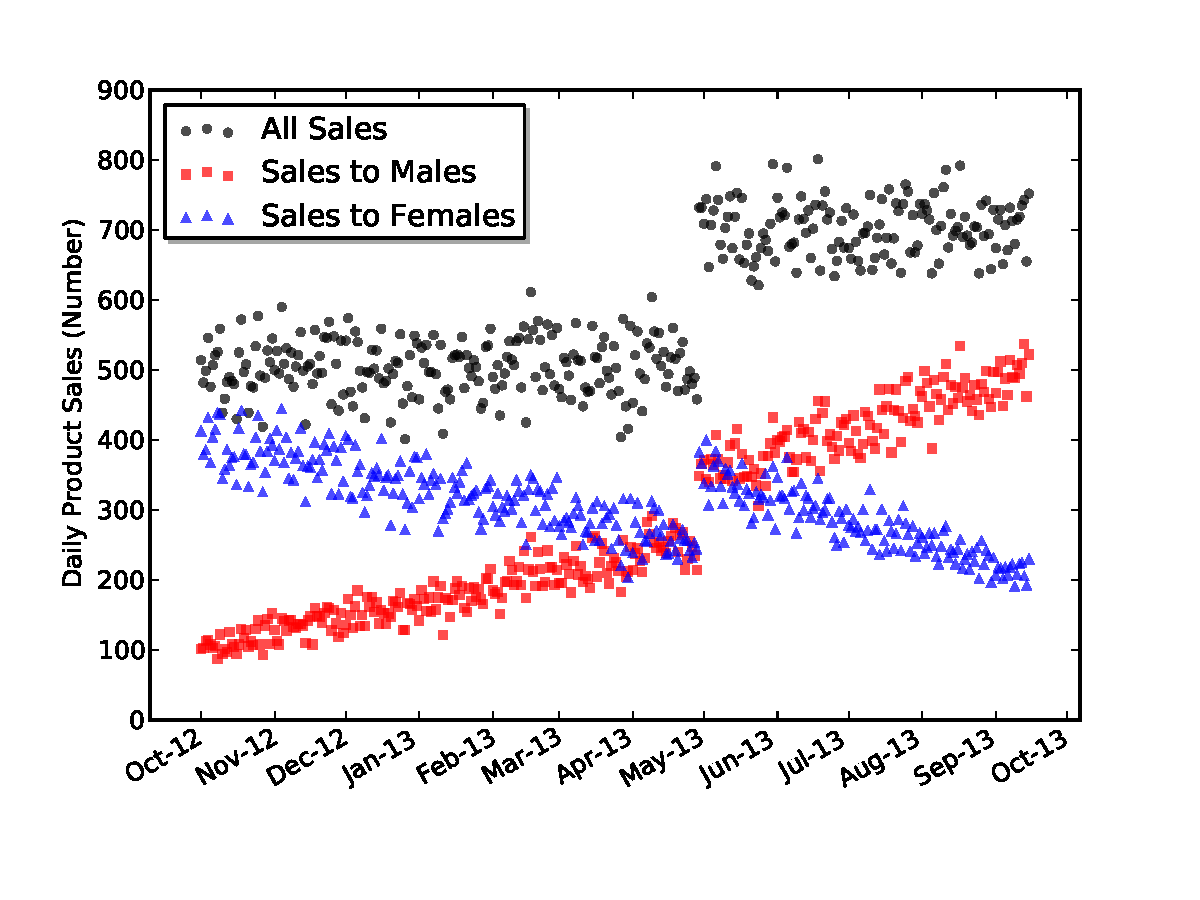
\includegraphics[scale=0.7]{../DailySalesComponentsFINAL.pdf}


Simple visual inspection shows that there is an ongoing shift in proportion of male to female sales: males are gaining product sales share. From here I hypothesize there is
some difference in product sales between male and female customers, but I must decide
if this long term shifting is tied to the jump at the date calculated above.

I note from inspection that at the time of sales jump, the male and females sales functions are equal or crossing.
{\bf Because the two populations' sales change at the same time, and by the same amount, I conclude that the jump is not linked to any shifting proportion of male to female sales.}
If a shifting proportion did effect the sudden change, I would have expected to see
one of the male or female components jump and not the other.

\section{Time of Day}

The original data's time stamp allows data to be sorted into the following four
categories: (12:00AM-6:00AM), (6:00AM-12:00PM), (12:00PM-6:00PM), (6:00PM-12:00AM),
 respectively called night, morning, afternoon, evening. I compiled sales by time of day
for the entire 50 weeks. The visual below shows percentages of total
sales from each time of day.


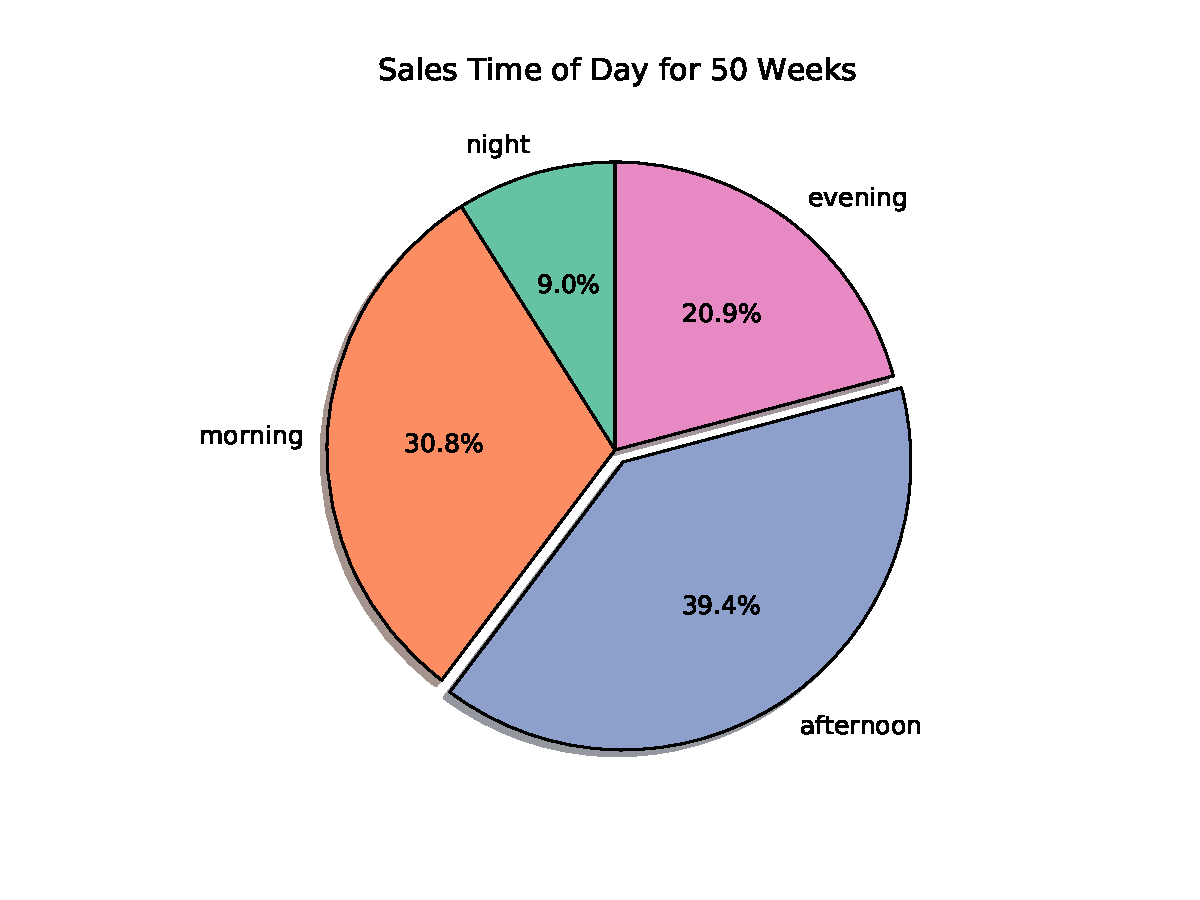
\includegraphics[scale=0.7]{../TimeOfDaySales.pdf}


The plot above shows a very coarse way of viewing time of day sales distribution.
I think it correctly answers the presented question but I would like to explore
an alternative: namely the time of day sales versus date over the entire date range.

Because sales environments can be sensitive to seasonal changes, holidays, natural disasters, policy changes etc., I am motivated to at least briefly inspect the time of
day sales on a daily scale. Such behaviors would be lost when the data is bucketed as coarsely as in the pie chart. I present the following plot as an additional "quick check" on the impact of time of day sales.

\begin{figure}[h!]
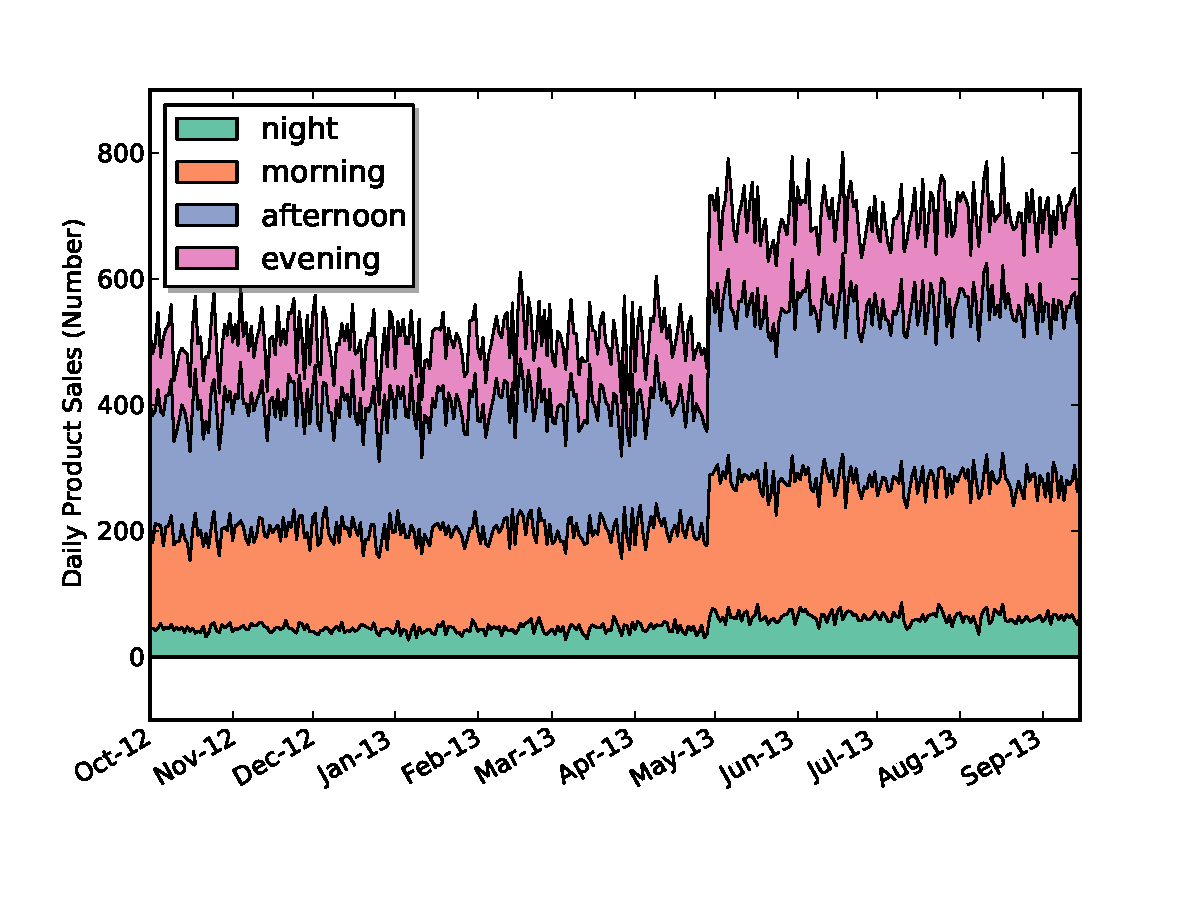
\includegraphics[scale=0.7]{../DataSalesTimeFilledLines.pdf}
\end{figure}

\section{In Closing}
If asked to guess the nature of these data,
I would suggest these data are generated using a Poisson distribution for each sex with a moving mean (a simple $y=mx+b$ or $\mu_i=m_ix + b_i$ line would suffice). The slopes of the lines are constructed via $m_{female}=-m_{male}$ so that the summed mean and variance are constant. The construction goes something like the following:

\begin{align}
\mu_{total} = \mu_{female} + \mu_{male}\\
\mu_{total} = b_{male} + b_{female}\\
\sigma^2_{total} = \sigma^2_{male} + \sigma^2_{female} \\
\sigma^2_{Poisson} \sim \mu \\
\sigma^2_{total} \sim \mu_{female} + \mu_{male}\\
\sigma^2_{total} \sim b_{male} + b_{female}\\ \nonumber
\end{align}
\noindent
Thus, there is a fixed total mean and total deviation.
Evidence for this appearss
in the plot above of the total sales, males sales, and female sales where the deviation grows for males, shrinks for females, and stays constant for total sales. 


The jump itself is likely a discontinuous change to the intercept of the lines
from which the gender sales are sampled. The time of day sales appear to be decided on a given day using random samples from fixed
percentage of that days already selected sales. {\bf It is indeed possible that these data are completely real, however I would
then conclude that sales are not sensitive to any holidays, so people are not giving
this product as a gift, which seems a small shame.}


Thanks for the opportunity to interview at 23andMe.

\end{document}
